\documentclass[tikz]{standalone}
\usepackage{pgfplots}
\pgfplotsset{compat=1.15}
\usepackage{mathrsfs}
\usetikzlibrary{arrows,calc}
\usepackage{tkz-euclide}

\pagestyle{empty}

\definecolor{AngleClr}{rgb}{0,0.39215686274509803,0}
\definecolor{ShapeClr}{rgb}{0.6,0.2,0}
\definecolor{LightGray}{RGB}{224, 224, 224}
\begin{document}

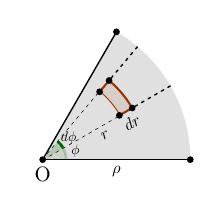
\begin{tikzpicture}[scale=.75]
\tkzSetUpLine[line width=1pt,color=black]
\tkzSetUpPoint[fill=black]

\tkzDefPoints{0/0/O}
\tkzDefPoint(30:1.5){A1}
\tkzDefPoint(50:1.5){A2}

\tkzDefPoint(30:1.75){B1}
\tkzDefPoint(50:1.75){B2}

\tkzDefPoint(0:2.5){C1}
\tkzDefPoint(60:2.5){C2}

\tkzDefPoint(30:2.5){D1}
\tkzDefPoint(50:2.5){D2}

\tkzFillSector[fill=LightGray](O,C1)(C2)

\tkzDrawSegments[line width=0.5pt,color=black](O,C1 O,C2)
\tkzDrawSegments[line width=0.5pt,color=black,dashed,dash pattern=on 1pt off 1.75pt](O,D1 O,D2)

\tkzDrawSegments[line width=0.75pt,color=ShapeClr](A1,B1 A2,B2)
\tkzDrawArc[line width=0.75pt,color=ShapeClr](O,B1)(B2)
\tkzDrawArc[line width=0.75pt,color=ShapeClr](O,A1)(A2)

\tkzFillSector[fill=ShapeClr,fill opacity=0.1](O,B1)(B2)
\tkzFillSector[fill=LightGray](O,A1)(A2)

\tkzFillAngle[fill=AngleClr,size=.4,fill opacity=0.1](C1,O,A1)
\tkzMarkAngle[line width=1pt,size=.4,color=AngleClr,opacity=0.2](C1,O,A1)
\tkzLabelAngle[pos=1.15,scale=0.5](C1,O,A1){$\phi$}

\tkzFillAngle[fill=AngleClr,size=.4,fill opacity=0.2](A1,O,A2)
\tkzMarkAngle[line width=1pt,size=.4,color=AngleClr](A1,O,A2)
\tkzLabelAngle[pos=1.15,scale=0.5](A1,O,A2){$d\phi$}

\tkzDrawPoints[size=2](O,A1,B1,C1,A2,B2,C2)
% \tkzLabelPoint[above](A){$\mathrm{A}$}

\tkzLabelPoint[below,scale=0.75](O){$\rm O$}
\tkzLabelSegment[below,scale=0.6,sloped,pos=0.75](O,A1){$r$}
\tkzLabelSegment[below,scale=0.6,sloped](A1,B1){$dr$}
\tkzLabelSegment[below,scale=0.6,sloped](O,C1){$\rho$}

\end{tikzpicture}
\end{document}
